\documentclass[10pt]{beamer}

\usepackage[utf8]{inputenc}
\usepackage[spanish]{babel}
\usepackage{graphicx}

\mode<presentation>
\usetheme{Madrid}
%\usecolortheme[RGB={111,73,135}]{structure}
\usecolortheme[RGB={128,0,0}]{structure}
%\usecolortheme[RGB={0,96,0}]{structure}
%\usecolortheme[RGB={200,0,200}]{structure}
%\usecolortheme[RGB={0,128,0}]{structure}
%\usecolortheme[RGB={0,0,128}]{structure}
\usefonttheme{serif}
\useinnertheme{rectangles}
\useoutertheme{split}

\setbeamercovered{transparent}

\title{Programación en Python}
\author{Jesús Espino García}
\date{7 de Noviembre de 2011}
\subject{Programación en Python}

\institute[Gul UC3M]{Gul UC3M Nov 2011\\
    
\includegraphics[height=1.5cm]{kaleidos.png}
}

\setcounter{tocdepth}{2}

\AtBeginSubsection[]
{
  \begin{frame}<beamer>{Indice}
    \tableofcontents[sectionstyle=show/shaded,subsectionstyle=show/shaded/hide]
  \end{frame}
}

\begin{document}

  \frame{\maketitle}

  \section*{Introducción}
  \begin{frame}{¿Qué es Python?}
    \begin{itemize}
      \item Lenguaje de programación.
      \item Creado por Guido Van Rossum en las navidades de 1989.
      \item Basado en ABC y Modula-3.
      \item En febrero de 1991 pasa a USENET.
      \item A partir de entonces el lenguaje no ha dejado de crecer.
      \item Actualmente coexisten dos versiones paralelas, 2.7 y 3.2.
    \end{itemize}
  \end{frame}
  
  \begin{frame}{¿Por qué Python?}
    \begin{center}
      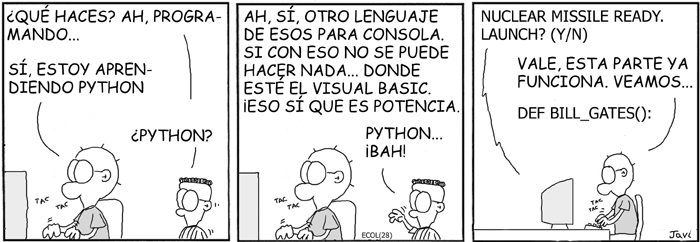
\includegraphics[height=4cm]{tiraecol_30.png}
    \end{center}
    \begin{itemize}
      \item Fácil de aprender.
      \item Sencillo de usar.
      \item Potente.
    \end{itemize}
  \end{frame}

  \begin{frame}{¿Por qué Python?}
    \begin{itemize}
      \item Libre (y gratis).
      \item Fácil de escribir.
      \item Fácil de leer.
      \item Fácil de mantener.
      \item De proposito general.
      \item Alto nivel.
      \item Orientado a objetos.
      \item Interpretado.
      \item Introspectivo.
    \end{itemize}
  \end{frame}

  \begin{frame}{¿Por qué Python?}
    \begin{itemize}
      \item Extensible.
      \item Completo.
      \item Dinamico.
      \item Robusto.
      \item Multiplataforma.
      \item Herencia multiple.
      \item List comprehesions.
      \item Funciones lambda.
      \item Clausuras.
      \item Bien documentado.
      \item Documentación integrada en el lenguage.
    \end{itemize}
  \end{frame}

  \begin{frame}{¿Quién lo usa?}
    \begin{itemize}
      \item Google.
      \item Microsoft.
      \item IBM.
      \item NASA.
      \item MIT.
      \item Yahoo!.
      \item HP.
      \item DOD.
      \item En resumen, todo el mundo.
    \end{itemize}
  \end{frame}
  
  \section*{Tipos básicos}
  \begin{frame}{Variables}
    \begin{itemize}
      \item Variables dinamicas.
      \item Principales tipos de datos:
      \begin{itemize}
        \item Booleanos (bool)
        \item Numericos (int, float, long, complex)
        \item Secuencias (str, unicode, list, tuple, bytearray)
        \item Sets (set, frozenset)
        \item Internos (module, function, instancemethod, instance, classobj)
      \end{itemize}
      \item Distincion entre mutables y no mutables:
      \begin{itemize}
        \item Mutable: Se cambia el valor del objeto. (Listas, ByteArrays y Sets)
        \item Inmutable: Al cambiar se sobreescribe el objeto. (Numericos, Booleanos, Strings, Tuplas y Fronzensets)
      \end{itemize}
    \end{itemize}
  \end{frame}

  \begin{frame}[containsverbatim]
    \frametitle{Listas}
    \begin{itemize}
        \item Son mutables.
        \item Se identifica por \verb+[]+
        \item Lista vacía: \verb+[]+
        \item Lista con datos homogeneos: \verb+[1,2,3,4]+
        \item Lista con datos heterogeneos: \verb+[1,(2,4),"cadena",["gul","linux","python"]]+
        \item Acceso a un elemento: \verb+lista[indice]+
        \item Listas dentro de listas: \verb+lista[indice1][indice2]..[indiceN]+
        \item Acceso desde el final: \verb+lista[-indice]+
    \end{itemize}
  \end{frame}

  \begin{frame}[containsverbatim]
    \frametitle{Tuplas}
    \begin{itemize}
        \item Son inmutables.
        \item Se identifica por \verb+()+
        \item Tupla vacía: \verb+()+
        \item Tupla de un elemento: \verb+(1,)+
        \item Tupla con datos homogeneos: \verb+(1,2,3,4)+
        \item Tupla con datos heterogeneos: \verb+(1,(2,4),"cadena",["gul","linux","python"])+
        \item Acceso a un elemento: \verb+tupla[indice]+
        \item Tuplas dentro de tuplas: \verb+tupla[indice1][indice2]..[indiceN]+
        \item Acceso desde el final: \verb+tupla[-indice]+
    \end{itemize}
  \end{frame}

  \begin{frame}[containsverbatim]
    \frametitle{Diccionario}
    \begin{itemize}
        \item Son mutables.
        \item Se identifica por \verb+{}+
        \item Diccionario vacío: \verb+{}+
        \item Diccionario con datos: \verb+{"nombre":"Jesus", "apellido":"Espino"}+
        \item Acceso a un elemento: \verb+diccionario[clave]+
        \item Diccionarios dentro de diccionarios: \verb+diccionario[clave1][clave2]..[claveN]+
    \end{itemize}
  \end{frame}

  \section*{Buceando dentro de python}
  \begin{frame}[containsverbatim]
    \frametitle{Introspección con dir()}
    \begin{itemize}
      \item Python es introspectivo.
      \item La funcion \verb+dir()+ nos muestra el contenido de un objeto.
      \item Metodos, atributos, modulos, todo son objetos y pueden estar
            contenidos unos en otros.
      \item \verb+dir()+ sin parametros nos muestra información del contexto principal.
    \end{itemize}
    \begin{verbatim}
>>> dir()
['__builtins__', '__doc__', '__name__', '__package__']
    \end{verbatim}
  \end{frame}

  \begin{frame}[containsverbatim]
    \frametitle{Obteniendo ayuda con help()}
    \begin{itemize}
      \item La función \verb+help()+ nos muestra la documentación de un objeto
      \item Por ejemplo \verb+help([].append)+
    \end{itemize}
    \begin{verbatim}
>>> help([].append)
Help on built-in function append:

append(...)
    L.append(object) -- append object to end
    \end{verbatim}
  \end{frame}

  \section*{Escribiendo código}
  \begin{frame}[containsverbatim]
    \frametitle{Indentado}
    \begin{itemize}
      \item En python en indentado es obligatorio.
      \item Forma parte de la sintaxis.
      \item Sirve para definir donde empieza y termina un bloque.
    \end{itemize}
    Ejemplo:
    \begin{verbatim}
if variable == 10:
    print "La variable es 10"
else:
    print "La variable no es 10"
    \end{verbatim}
  \end{frame}
  
  \begin{frame}[containsverbatim]
    \frametitle{Condiciones}
    \begin{verbatim}
if variable == 10:
    print "La variable es 10"
elif variable == 20:
    print "La variable es 20"
else:
    print "La variable no es ni 10, ni 20"
    \end{verbatim}
  \end{frame}

  \begin{frame}[containsverbatim]
    \frametitle{Bucle while}
    \begin{verbatim}
while value < 10:
    print value
    value += 1
else:
    print "End"
    \end{verbatim}
    \begin{itemize}
      \item \verb+break+ sale el bucle.
      \item \verb+continue+ pasa a la siguiente iteración.
    \end{itemize}
  \end{frame}

  \begin{frame}[containsverbatim]
    \frametitle{Bucle for}
    \begin{verbatim}
for value in lista:
    print value
else:
    print "End"
    \end{verbatim}
    \begin{itemize}
      \item \verb+break+ sale el bucle.
      \item \verb+continue+ pasa a la siguiente iteración.
    \end{itemize}
  \end{frame}

  \begin{frame}[containsverbatim]
    \frametitle{Definición de funciones}
    \begin{verbatim}
def funcion(arg1, arg2="default", *args, **kwargs):
    'Documentación de la funcion'
    print arg1
    print arg2
    print args
    print kwargs
    return "Valor"
function(1)
function(1,2,3,4,prueba=5)
    \end{verbatim}
  \end{frame}

  \section*{Escribiendo programas}

  \begin{frame}[containsverbatim]
    \frametitle{Ficheros de python}
    \begin{verbatim}
#!/usr/bin/env python
# -*- coding: utf-8 -*-

def mifuncion():
    print "Hola Mundo"

if __name__=='__main__':
    mifuncion()
    \end{verbatim}
  \end{frame}

  \begin{frame}[containsverbatim]
    \frametitle{Entrada por teclado}
    \begin{verbatim}
x=input("Obtener valor: ")
pritn x
y=raw_input("Obtener valor: ")
print y
    \end{verbatim}
  \end{frame}

  \begin{frame}[containsverbatim]
    \frametitle{Parámetros del programa}
    \begin{verbatim}
import sys
nombre_de_script = sys.argv[0]
primer_parametro = sys.argv[1]
segundo_parametro = sys.argv[2]
    \end{verbatim}
  \end{frame}

  \begin{frame}[containsverbatim]
    \frametitle{Acceso a ficheros}
    \begin{verbatim}
fichero = open('fichero.txt','r')
datos = fichero.read()
fichero.close()
fichero2 = open('fichero2.txt','w')
fichero2.write(datos)
fichero2.close()
    \end{verbatim}
  \end{frame}

  \begin{frame}[containsverbatim]
    \frametitle{Clases}
    \begin{verbatim}
class MiClase(object):
    dato = None

    def set_dato(self, dato):
        self.dato=dato

    def display(self):
        print self.dato

    def get_dato(self):
        return self.dato
    \end{verbatim}
  \end{frame}

  \begin{frame}[containsverbatim]
    \frametitle{Herencia}
    \begin{verbatim}
class OtraClase(MiClase):
    def display(self):
        print "El valor actual es %s" % (self.dato)
    \end{verbatim}
  \end{frame}

  \begin{frame}[containsverbatim]
    \frametitle{Metodos especiales}
    \begin{itemize}
      \item \verb+__init__+: Constructor.
      \item \verb+__del__+: Destructor.
      \item \verb+__add__+: Operador de suma.
      \item \verb+__or__+: Operador Or lógico.
      \item \verb+__getitem__+: Indexación.
      \item \verb+__setitem__+: Asignación indexada.
      \item \verb+__getslice__+: Seleccionar una parte.
      \item \verb+__repr__+: Para salida por pantalla.
      \item \verb+__len__+: Longitud.
      \item \verb+__cmp__+: Comparación.
      \item \verb+__unicode__+: Representación unicode.
      \item \verb+__str__+: Representación en string.
    \end{itemize}
  \end{frame}

  \begin{frame}[containsverbatim]
    \frametitle{Excepciones}
    \begin{verbatim}
try:
    x = int(variable)
except ValueError:
    print "La variable no es un entero"
else:
    print "Todo ha ido ok"
finally:
    print "Pase lo que pase se ejecuta esto"

raise "Excepcion personalizada"
    \end{verbatim}
  \end{frame}

  \begin{frame}[containsverbatim]
    \frametitle{Módulos}
    \begin{itemize}
      \item Bloques de código que agrupan funciones, clases y variables.
      \item Pueden ser ficheros .py.
      \item Pueden ser directorios que contengan un \verb+__init__.py+.
    \end{itemize}
    \begin{verbatim}
fichero1.py:
def mifuncion():
    print "Hola Mundo"

fichero2.py
import fichero1
fichero1.mifuncion()
    \end{verbatim}
  \end{frame}

  \section*{Para terminar}
  
  \begin{frame}{Referencias}
    \begin{itemize}
      \item Proyecto python: http://www.python.org.
      \item Documentación de python: http://docs.python.org.
      \item Python-ES: python-es@python.org
    \end{itemize}
  \end{frame}

  \begin{frame}{Dudas}
    \begin{center}
      \dots
    \end{center}
  \end{frame}

\end{document}
